\documentclass{replab}
\usepackage{lipsum}

% --- Información del documento ---
\title{}
\author{Zahid Medrano Flores}
\subtitle={Análisis del Transtorno del Sueño}
\subject={\textit{Temas Selectos en Biomatemáticas.} \textbf{Introducción a la Ciencia de Datos.}}

\setlength{\columnsep}{14pt}

% --- Archivo de bibliografía ---
\addbibresource{ref.bib}

% --- Inicio del documento ---
\begin{document}
	
	\pagestyle{fancy}
	\unspacedoperators
	
% --- Título ---
\selectlanguage{spanish}
	
% --- Cuerpo del reporte ---

\twocolumn[
    \begin{center}
        \maketitle

            {\begin{tcolorbox}[colframe=white, colback=principaldos, arc=6pt]
				\begin{onecolabstract}

                    Este reporte aborda el problema de los trastornos del sueño a través del análisis de un dataset, buscando no solo explorar las características y patrones presentes en los datos, sino también proponer y evaluar la aplicación de técnicas analíticas y modelos de Machine Learning como herramientas potenciales para arrojar luz sobre este gran problema de salud.
    
                \end{onecolabstract}
			\end{tcolorbox}}
    \end{center}
]

\bigskip
	
\section{Introducción}

El sueño es una parte muy importante de la vida y salud humana, es tan vital y necesario como una buena nutrición o actividad física regular. En este breve periodo que tenemos, nuestro cuerpo y mente se recuperan, se consolida la memoria, se regula el estado de ánimo y algunas otras funciones esenciales que tenemos para el bienestar integral. Sin embargo, a nivel mundial se presentan transtornos del sueño, los cuales son condiciones que afectan la calidad del mismo.

Los trastornos del sueño no son simplemente una molestia; representan un problema de salud pública creciente con muchas implicaciones a nivel individual y social. La falta crónica de sueño o un sueño de mala calidad está asociado con un mayor riesgo de desarrollar una amplia gama de problemas de salud, incluyendo enfermedades cardiovasculares, diabetes, obesidad, trastornos de salud mental (como depresión y ansiedad) y una disminución inmunológica. Además, tenemos que los tipos de transtornos tienen una amplia gama de síntomas. Los transtornos mas comunes incluyen el \textit{insomnio}, la \textit{narcolepsia}, la \textit{apnea} (dificultades respiratorias), etc.  Estos padecimientos tienen tanto impacto, que llega a nuestra vida diaria, afectando nuestra concentración, toma de decisiones o rendimiento en general.

La complejidad de los trastornos del sueño se debe a su diversa naturaleza y en la variedad de agentes que pueden contribuir a ellos, desde hábitos de vida y condiciones médicas subyacentes hasta factores genéticos y ambientales. Tradicionalmente, el diagnóstico y manejo se han basado en la evaluación clínica, cuestionarios y estudios especializados. Sin embargo, la creciente disponibilidad de datos sobre patrones de sueño, estilos de vida y salud, así como los avances en ciencia de datos y Machine Learning, abren nuevas puertas para comprender mejor estos trastornos, identificar poblaciones en riesgo y desarrollar mejores enfoques para su detección y tratamiento.

	\section{Desarrollo}

En un proyecto de Ciencia de Datos, el objetivo principal es construir modelos matemáticos y computacionales que tienen la capacidad de ``aprender'' a partir de datos existentes, para poder realizar prediccciones sobre datos nuevos.

    \subsection{Análisis exploratorio}

En un análisis exploratorio se busca analizar y de alguna forma, manipular nuestro conjunto de datos, para poder obtener mejores resultados en nuestros modelos predictivos.

Nuestro proceso del análisis exploratorio fue el siguiente

1. Carga de datos. Se carga el dataset y se realiza un análisis exploratorio inicial, donde entendemos la estructura de los datos, las variables y la distribución de clases (los transtornos del sueño) presentes.

2. Limpieza. Se tratan los valores nulos, se corrigen errores y las varias inconsistencias que se presenten a lo largo del dataset.

3. Transformación. En esta parte, realizamos distintos procesos para transformar los datos. Se realiza un manejo de variables categóricas, una normalización o escalado de las variables numéricas, entre otros procesos.

4. Oversampling. Si nuestro dataset es muy pequeño, y lo vemos necesario, se realiza un sobremuestreo para aumentar el número de ejemplos de la clase más pequeña en un conjunto de datos desequilibrado. Esto es opcional, pero muchas veces ayuda.

\subsection{Split}

A partir de nuestro dataset completo, se realiza una división de nuestro conjunto para el entrenamiento (train) y las pruebas o inferencia (test). Una división común es de 70 / 30 para el entrenamiento y el test respectivamente.

    \subsection{Modelos}

Hay una gran variedad de modelos, los cuales se escogen de acuerdo al problema que se esté atacando. En nuestro caso se trata de un proyecto enfocado en la clasificación de transtornos del sueño. Por lo tanto tenemos algunas opciones.

        \begin{itemize}[itemsep=-2pt]

            \item \textbf{Logistic Regression:}
            Es un algoritmo de clasificación lineal que modela la probabilidad de que una instancia pertenezca a una clase particular. Funciona aplicando una función logística (sigmoide) a una combinación lineal de las características de entrada. \cite{cramer}

            \item \textbf{Gradient Boosting Machine (GBM):}
            Es una técnica de boosting que construye un modelo predictivo en etapas, y generaliza la optimización de la función de pérdida utilizando el descenso de gradiente. \cite{friedman}

            \item \textbf{eXtreme Gradient Boost:}
            Es una implementación optimizada y muy eficiente del algoritmo Gradient Boosting. Se destaca por su velocidad y rendimiento. Construye una serie de árboles de decisión de forma secuencial, donde cada nuevo árbol intenta corregir los errores anteriores. \cite{chen}

            \item \textbf{K-Nearest Neighbors (KNN):}
            Para clasificar un nuevo punto de datos, KNN encuentra los '$k$' puntos de datos más cercanos en el espacio de características (basado en una métrica de distancia) y asigna la clase más común. \cite{cunningham}

            \item \textbf{C-Support Vector (SVC):}
            Es un tipo de SVM utilizada para tareas de clasificación. Encuentra el hiperplano óptimo que mejor separe las diferentes clases en el espacio de características, maximizando el margen entre los puntos de datos de las clases más cercanas a ese hiperplano (los vectores de soporte). \cite{novakovic}

            \item \textbf{Random Forest:}
            Es un algoritmo de aprendizaje por conjunto (ensemble learning) que funciona construyendo un gran número de árboles de decisión durante la fase de entrenamiento. En la clasificación, combina las predicciones de todos los árboles para determinar la clase. \cite{cutler}

        \end{itemize}


\section{Resultados}

En esta sección se presentan los resultados obtenidos para cada uno de los modelos que se probaron.

    \subsection{Logistic Regression}

La complejidad de implementación de este modelo no es tan grande, no tiene tantos hiperparámetros que se puedan cambiar de manera rápida y que sean de gran impacto. Por lo tanto el modelo es bastante fácil de aplicar.

A continuación se presenta la figura \ref{fig:matrizLR} con la matriz de confusión para poder observar el comportamiento que presenta el modelo al momento de predecir los transtornos del sueño.

\begin{figure}[hbt!]
    \centering
    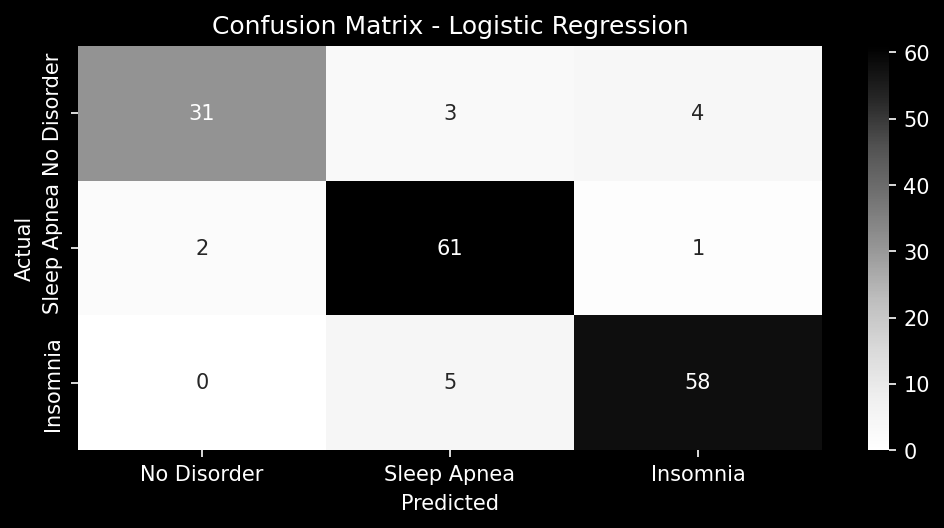
\includegraphics[width=0.85\columnwidth]{imagenes/LogisticRegression.png}
    \caption{Matriz de confusión para el modelo de Logistic Regression.}
    \label{fig:matrizLR}
\end{figure}

Este modelo presentó una precisión del $\approx 91.07\%$ y una exactitud igualmente buena de $90.90\%$.

    \subsection{Gradient Boosting Machine}

De manera similar, la implementación del este modelo se realizó de manera simple. De hiperparámetros no hay mucho que cambiar, pero se utilizaron mas n - estimadores para probar el comportamiento que presentara.

La figura \ref{fig:matrizGBM} que se presenta a continuación, muestra la matriz de confusión, con la cual vemos que tan bien puede predecir nuestras clases de transtornos.

\begin{figure}[hbt!]
    \centering
    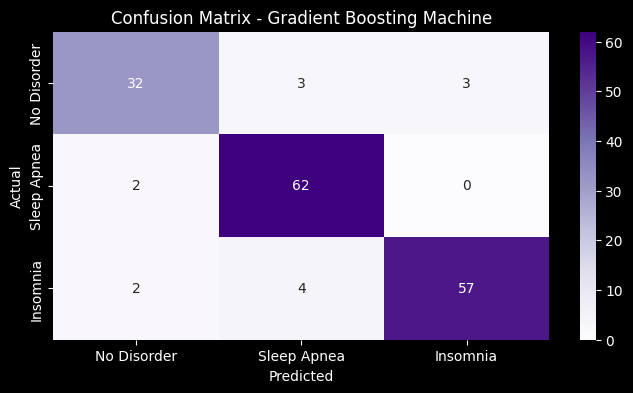
\includegraphics[width=0.85\columnwidth]{imagenes/GBM.png}
    \caption{Matriz de confusión para el modelo GBM.}
    \label{fig:matrizGBM}
\end{figure}

El modelo demostró ser capaz de una precisión del $\approx 91.59 \%$ con una exactitud del $91.51$.

    \subsection{eXtreme Boosting Machine}

El XGBoost es una libreria altamente optimizada, que implementa de una manera mas eficiente y flexible el Gradien Boosting. Por lo tanto, no hay muchos parámetros que probar. Entonces es una simple aplicación de la libreria sobre nuestro dataset.

La matriz de confusión se encuentra en la figura \ref{fig:matrizXGB}, la cual se presenta a continuación.

\begin{figure}[hbt!]
    \centering
    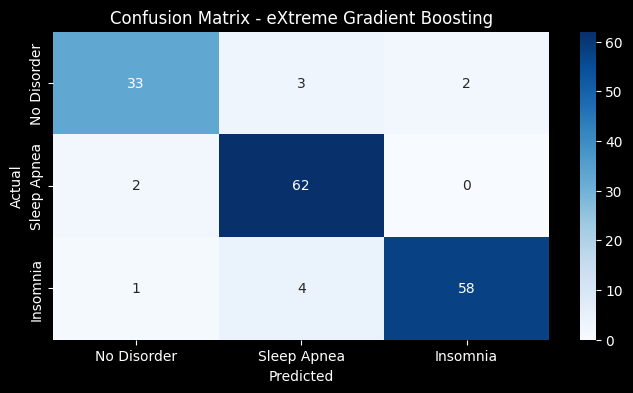
\includegraphics[width=0.85\columnwidth]{imagenes/XGB.png}
    \caption{Matriz de confusión para el modelo utilizando xGBoost.}
    \label{fig:matrizXGB}
\end{figure}

El modelo obtuvo una precisión de $\approx 92.87\%$ con una exactitud del $92.72\%$

    \subsection{K-Nearest Neighbors}

En el modelo de KNN se utilizaron 5 vecinos, y se probaron los diversos algoritmos. Se optó por el algoritmo `brute', el cual como el nombre nos indica, busca los vecinos por fuerza bruta. Todo lo demás se dejó en su parámetro predeterminado.

La figura \ref{fig:matrizKNN} nos muestra la matriz de confusión correspondiente a nuestro modelo.

\begin{figure}[hbt!]
    \centering
    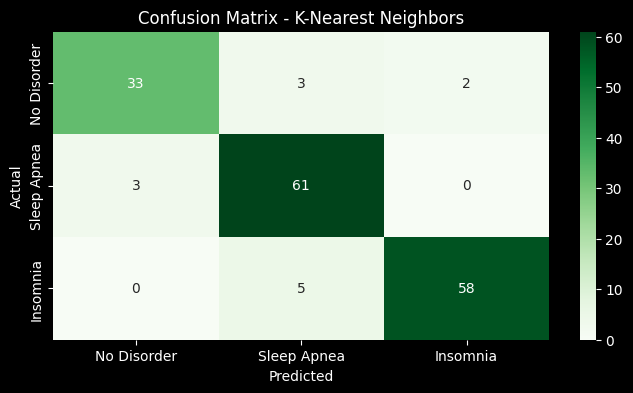
\includegraphics[width=0.85\columnwidth]{imagenes/KNN.png}
    \caption{Matriz de confusión para el modelo de K-Nearest Neighbors.}
    \label{fig:matrizKNN}
\end{figure}

El modelo nos arrojó una precisión de $\approx 92.31\%$ con una exactitud del $91.12\%$.

    \subsection{C-Supoort Vector}

El SVC es un tipo de implementación del modelo de SVM. Aquí el único hiperparámetro que se ajustó fue el kernel utilizado, quedándonos con el `poly' o polinómico.

La matriz de confusión se muestra en la figura \ref{fig:matrizSVC} a continuación.

\begin{figure}[hbt!]
    \centering
    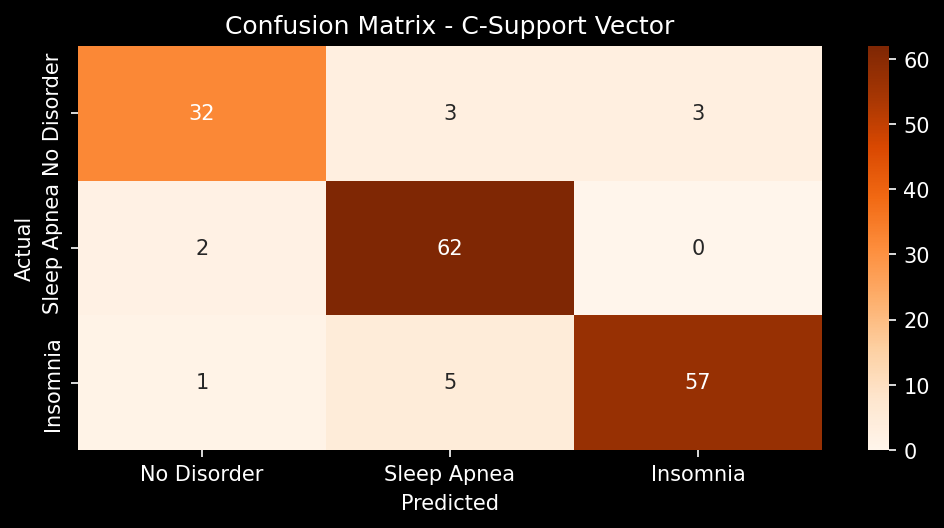
\includegraphics[width=0.85\columnwidth]{imagenes/SVC.png}
    \caption{Matriz de confusión para el modelo de SVC.}
    \label{fig:matrizSVC}
\end{figure}

El modelo presentó una precisión del $\approx 91.68\%$ con una exactitud de alrededor del $91.51\%$.

    \subsection{Random Forest}

Finalmente, tenemos el RandomForest. En este modelo si hay varios hiperparámetros que se pueden optimizar, pero, el uso de un GridSearch o un RandomSearch requiere de mucho poder computacional que honestamente no vale la pena. Por lo tanto, se optó por utilizar la cantidad de 150 árboles y una profundiad de los mismos de 5.

La figura \ref{fig:matrizRNF} que se presenta a continuación, nos muestra la matriz de confusión correspondiente al RandomForest.

\begin{figure}[hbt!]
    \centering
    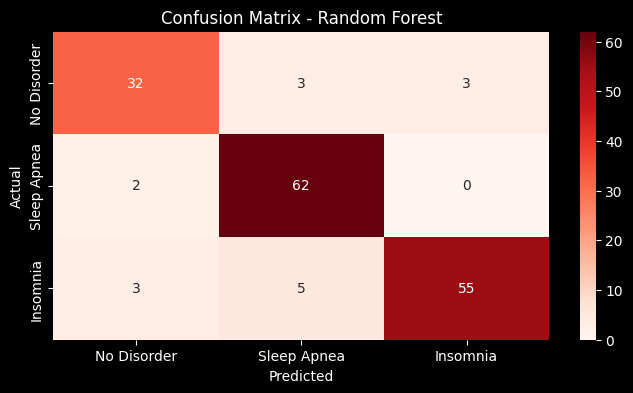
\includegraphics[width=0.85\columnwidth]{imagenes/RandomForest.png}
    \caption{Matriz de confusión para el modelo utilizando un RandomForest.}
    \label{fig:matrizRNF}
\end{figure}

El modelo muestra una precisión de $\approx 89.92\%$ con una exactitud del $89.69\%$.

\section{Análisis y Discusión}

Como ya se comentó, el objetivo principal del reporte es abordar el problema de los trastornos del sueño mediante el análisis de un dataset y la aplicación de diversas técnicas de Machine Learning para su clasificación. Se realizó un proceso de análisis exploratorio que incluyó la carga, limpieza y transformación de los datos. Posteriormente, el dataset se dividió en conjuntos de entrenamiento y prueba. Se evaluaron seis modelos de clasificación: Logistic Regression, Gradient Boosting Machine (GBM), eXtreme Gradient Boost (XGBoost), K-Nearest Neighbors (KNN), C-Support Vector (SVC) y Random Forest.

Los resultados obtenidos para cada modelo en términos de precisión y exactitud fueron los siguientes:

\begin{itemize}
    \item \textbf{Logistic Regression:} Precisión $\approx 91.07\%$ y exactitud $\approx 90.90\%$. La implementación de este modelo fue sencilla con pocos hiperparámetros de gran impacto.
    \item \textbf{Gradient Boosting Machine (GBM):} Precisión $\approx 91.59\%$ y exactitud $\approx 91.51\%$. La implementación también fue simple, ajustando el número de estimadores.
    \item \textbf{XGBoost:} Precisión $\approx 92.87\%$ y exactitud $\approx 92.72\%$. Este modelo, una implementación optimizada de Gradient Boosting, mostró un alto rendimiento y velocidad.
    \item \textbf{KNN:} Precisión $\approx 92.31\%$ con una exactitud del $91.12\%$. Se utilizaron 5 vecinos y el algoritmo 'brute'.
    \item \textbf{SVC:} Precisión $\approx 91.68\%$ y exactitud $\approx 91.51\%$. Se ajustó el kernel a 'poly' (polinómico).
    \item \textbf{Random Forest:} Precisión $\approx 89.92\%$ y exactitud $\approx 89.69\%$. Se configuró con 150 árboles y una profundidad de 5, considerando que la optimización exhaustiva de hiperparámetros no compensaba el costo computacional.
\end{itemize}

Las matrices de confusión (Figura \ref{fig:matrizLR}, Figura \ref{fig:matrizGBM}, Figura \ref{fig:matrizXGB}, Figura \ref{fig:matrizKNN}, Figura \ref{fig:matrizSVC}, Figura \ref{fig:matrizRNF}) proporcionan una visualización detallada del desempeño de cada modelo en la clasificación de los diferentes trastornos del sueño (Insomnia, Sleep Apnea, No Disorder).

En general, todos los modelos presentaron un desempeño aceptable en la clasificación de los trastornos del sueño, todos con una precisión y exactitud por encima del 89\%. Destaca el modelo XGBoost con la mayor precisión y exactitud, lo que sugiere que las técnicas de boosting son particularmente efectivas para este problema con el dataset utilizado. El modelo Random Forest, a pesar de ser un método robusto, obtuvo las métricas ligeramente más bajas. La elección del modelo más adecuado dependerá también de otros factores como el tiempo de entrenamiento y la capacidad de obtener nuevos datos.

\section{Conclusiones}

El análisis de los trastornos del sueño a través de técnicas de ciencia de datos y Machine Learning demuestra ser una herramienta muy útil, nos ayuda a identificar y potencialmente mejorar los enfoques de detección y tratamiento de estas condiciones de salud pública. Los modelos evaluados en este reporte mostraron una capacidad significativa para clasificar los diferentes tipos de trastornos del sueño presentes en el dataset.

Específicamente, el modelo de eXtreme Gradient Boost (XGBoost) nos mostró el mejor rendimiento en términos de precisión y exactitud. Esto subraya el potencial de este tipo de algoritmos de boosting para la aplicación en problemas similares.

Si bien los resultados son buenos, es importante considerar que el desempeño de los modelos puede depender en gran medida de la calidad y las características que presente nuestro dataset utilizado. La manera mas óptima de mejorar estos procesos sería explorar la aplicación de estas técnicas en conjuntos de datos más grandes, así como la optimización más profunda de los hiperparámetros de cada modelo para mejorar al máximo su rendimiento.

Este reporte es un acercamiento breve a la utilidad que tiene el Machine Learning en diversas aplicaciones. No se espera que los modelos sean perfectos, pero, si es importante saber que existen herramientas que pueden ayudarnos a mejorar muchos aspectos de nuestar vida cotidiana.

% ----------------------------------------------------------------

\DeclareFieldFormat{labelnumberwidth}{\mkbibbrackets{#1}}
\defbibenvironment{bibliography}
  {\list
     {\printtext[labelnumberwidth]{%
      \printfield{labelprefix}%
      \printfield{labelnumber}}}
     {\setlength{\labelwidth}{\labelnumberwidth}%
      \setlength{\leftmargin}{\labelwidth}%
      \setlength{\labelsep}{\biblabelsep}%
      \addtolength{\leftmargin}{\labelsep}%
      \setlength{\itemsep}{\bibitemsep}%
      \setlength{\parsep}{\bibparsep}}%
      \renewcommand*{\makelabel}[1]{\hss##1}}
  {\endlist}
  {\item}

\printbibliography[heading=bibintoc]

\end{document}